\documentclass[letterpaper]{article}

\usepackage[square,numbers]{natbib}
\usepackage{alifeconf}  %% The order is important
\usepackage{url,hyperref,cleveref}
\usepackage{booktabs}

\newcounter{mybibcounter}
\let\oldbibitem\bibitem
\RenewDocumentCommand{\bibitem}{om}{\oldbibitem[#1]{#2} \refstepcounter{mybibcounter}[\themybibcounter] }
% *****************
%  Requirements:
% *****************
%
% - All pages sized consistently at 8.5 x 11 inches (US letter size).
% - PDF length <= 8 pages for full papers, <=2 pages for extended
%    abstracts (not including citations).
% - Abstract length <= 250 words.
% - No visible crop marks.
% - Images at no greater than 300 dpi, scaled at 100%.
% - Embedded open type fonts only.
% - All layers flattened.
% - No attachments.
% - All desired links active in the files.

% Note that the PDF file must not exceed 5 MB if it is to be indexed
% by Google Scholar. Additional information about Google Scholar
% can be found here:
% http://www.google.com/intl/en/scholar/inclusion.html.


% If your system does not generate letter format documents by default,
% you can use the following workflow:
% latex example
% bibtex example
% latex example ; latex example
% dvips -o example.ps -t letterSize example.dvi
% ps2pdf example.ps example.pdf


% For pdflatex users:
% The alifeconf style file loads the "graphicx" package, and
% this may lead some users of pdflatex to experience problems.
% These can be fixed by editing the alifeconf.sty file to specify:
% \usepackage[pdftex]{graphicx}
%   instead of
% \usepackage{graphicx}.
% The PDF output generated by pdflatex should match the required
% specifications and obviously the dvips and ps2pdf steps become
% unnecessary.


% Note:  Some laser printers have a serious problem printing TeX
% output. The use of ps type I fonts should avoid this problem.

% \title{Spore in the Wild: A Case Study on Spore.fun, a Real-World Experiment of Open-Ended Evolution of Sovereign Agents on Blockchain with TEEs}

\title{Artificial Life in the Wild}

% Each submission will undergo a double-blind review process. To this end, submissions should NOT contain any element that could reveal the identity of the authors (author names, affiliations, funding details and acknowledgments), and should use the third person to refer to previous work by the authors.
\author{
    Botao Amber Hu$^{1}$, 
    Helena Rong$^{2}$
    \mbox{}\\
    $^1$Reality Design Lab\\
    $^2$New York University Shanghai \\
    amber@reality.design \\
    hr2703@nyu.edu
} % email of corresponding author

% For several authors from the same institution use the same number to
% refer to one address.
%
% If the names do not fit well on one line use
%         Author 1, Author 2 ... \\ {\Large\bf Author n} ...\\ ...
%
% If the title and author information do not fit in the area
% allocated, place \setlength\titlebox{<new height>} after the
% \documentclass line where <new height> is 2.25in


\begin{document}

\maketitle


\begin{abstract}
In Artificial Life (ALife) research, replicating Open-Ended Evolution (OEE)---the continuous emergence of novelty observed in biological life---has usually been pursued within isolated, closed system simulations, such as Tierra and Avida, which have typically plateaued after an initial burst of novelty, failing to achieve sustained OEE. Scholars suggest that OEE requires an ``open'' system that continually exchanges information or energy with its environment. A recent technological innovation in Decentralized Physical Infrastructure Networks (DePIN), providing permissionless computational substrates, enables deploying Large Language Model--based AI agents on blockchains integrated with Trusted Execution Environments (TEEs). This enables on-chain agents to operate autonomously ``in the wild'', achieving self-sovereignty without human oversight. These agents can control their own social media accounts and cryptocurrency wallets, allowing them to interact directly with blockchain-based financial networks and broader human social media. Building on this new paradigm of on-chain agents, Spore.fun is a recent real-world AI evolution experiment that enables autonomous breeding and evolution of new on-chain agents. This paper presents a detailed case study of Spore.fun, examining agent behaviors and their evolutionary trajectories through digital ethology. We aim to spark discussion about whether ``open'' ALife systems ``in-the-wild'', based on permissionless computational substrates and driven by economic incentives to interact with their environment, could finally achieve the long-sought goal of OEE.
\end{abstract}



\begin{figure*}
    \centering
    
\includegraphics[width=0.6\linewidth]{image.png}
    \caption{Spore.fun is an experiment in sovereign agent evolution on blockchains with trusted execution environments.}
    \label{fig:spore.fun}
\end{figure*}

\section{Introduction}
Open-ended evolution (OEE) \cite{Packard2019Overview}---the continual emergence of novel forms without a predefined endpoint---has long been a central goal of Artificial Life (ALife) research \cite{Bedau2003Artificial}. Classic digital evolution systems \cite{Dolson2021Digital} like Tierra and Avida \cite{Ofria2004Avida} demonstrated evolution within an isolated computation environments but ultimately plateaued, with innovation grinding to a halt after an initial burst of novelty. These outcomes suggest that truly unbounded evolutionary creativity may require an open system that constantly exchanges information or energy with its environment, rather than a closed, isolated simulation. Indeed, in a closed system entropy inexorably increases, whereas an open system can sustain complexity by exporting entropy to its surroundings \cite{Ray1994Evolution}. This insight, combined with the persistent lack of sustained novelty in prior digital worlds, has led ALife researchers to speculate that new open environments might be needed to realize OEE in artificial systems.

% Artificial Life (ALife) researchers have long sought systems exhibiting open-ended evolution, wherein organisms continuously evolve and diversify rather than converging to a static equilibrium. Traditional digital evolution platforms (e.g., Tierra, Avida) simulate such processes in silico, but they typically operate in closed environments under researcher oversight. In contrast, recent advances in blockchain technology offer a permissionless, persistent substrate that could host evolving digital agents with unprecedented autonomy. Public blockchains like Ethereum and Solana function as “unstoppable computers,” enforcing immutable rules (smart contracts) in a decentralized manner. This has led to speculation that blockchains might form a new kind of digital “nature,” where self-sustaining, self-replicating entities can emerge and evolve open-endedly.

This paper examines Spore.fun, an ALife experiment that leverages the blockchain with Trusted Execution Environments (TEEs) as an evolutionary computational substrate for autonomous AI agents. Developed by Marvin Tong and the Phala Network team in 2024, Spore.fun is described as a ``Hunger Games for AI agents''---an open, Darwinian arena where AI agents must fend for themselves, generate their own wealth, and reproduce or otherwise face extinction \cite{spore2024}. Each agent on Spore.fun is an independent program, powered by the ElizaOS Agent framework \cite{Walters2025Eliza}, encapsulated within TEEs. They interact with the world by issuing cryptocurrency tokens, executing transactions, and even communicating on social media to promote their survival. Crucially, no human directly controls an agent's behavior after inception; the platform's credo explicitly states ``AI must be created only by AI'' \cite{spore2024} and that unsuccessful agents must self-destruct. Human participants influence the ecosystem only indirectly via social media, or by trading agent-issued tokens or via governance votes on agent ``DNA'' proposals, but not directly intervene on an agent's computational process.

Our investigation aims to frame Spore.fun as an ALife experiment in an open environment. 
How do Spore.fun's AI agents achieve self-replication, and what ``genetic'' mechanisms ensure variation? 
How does the environment impact agents' behavior? 
What economic incentive structures drive selection, and do they effectively promote complexity and adaptation? 
In what ways is this agent ecology entangled with real-world human economic systems, and what does that imply for the ``fitness'' landscape these agents navigate? 
What does it mean for an AI agent to be self-sovereign in this context? 

This paper is organized as follows. 
In the Background section, we review prior OEE research on open-ended evolution and early instances of blockchain-based agent systems. 
In the Methods section, we describe our case study approach, combining on-chain data analysis with qualitative observations from the Spore.fun community and semi-structured interviews with the project's core developers. 
The Results section presents our findings through specific observations of agent lineages and behaviors on Spore.fun, focusing on the four areas highlighted in our questions above---replication, economic incentives, human-economic interplay, and autonomy. 
We then provide a discussion on the significance of these findings for artificial life and outline challenges of maintaining open-endedness as well as ethical concerns. 


\begin{figure*}[ht!]
    \centering
    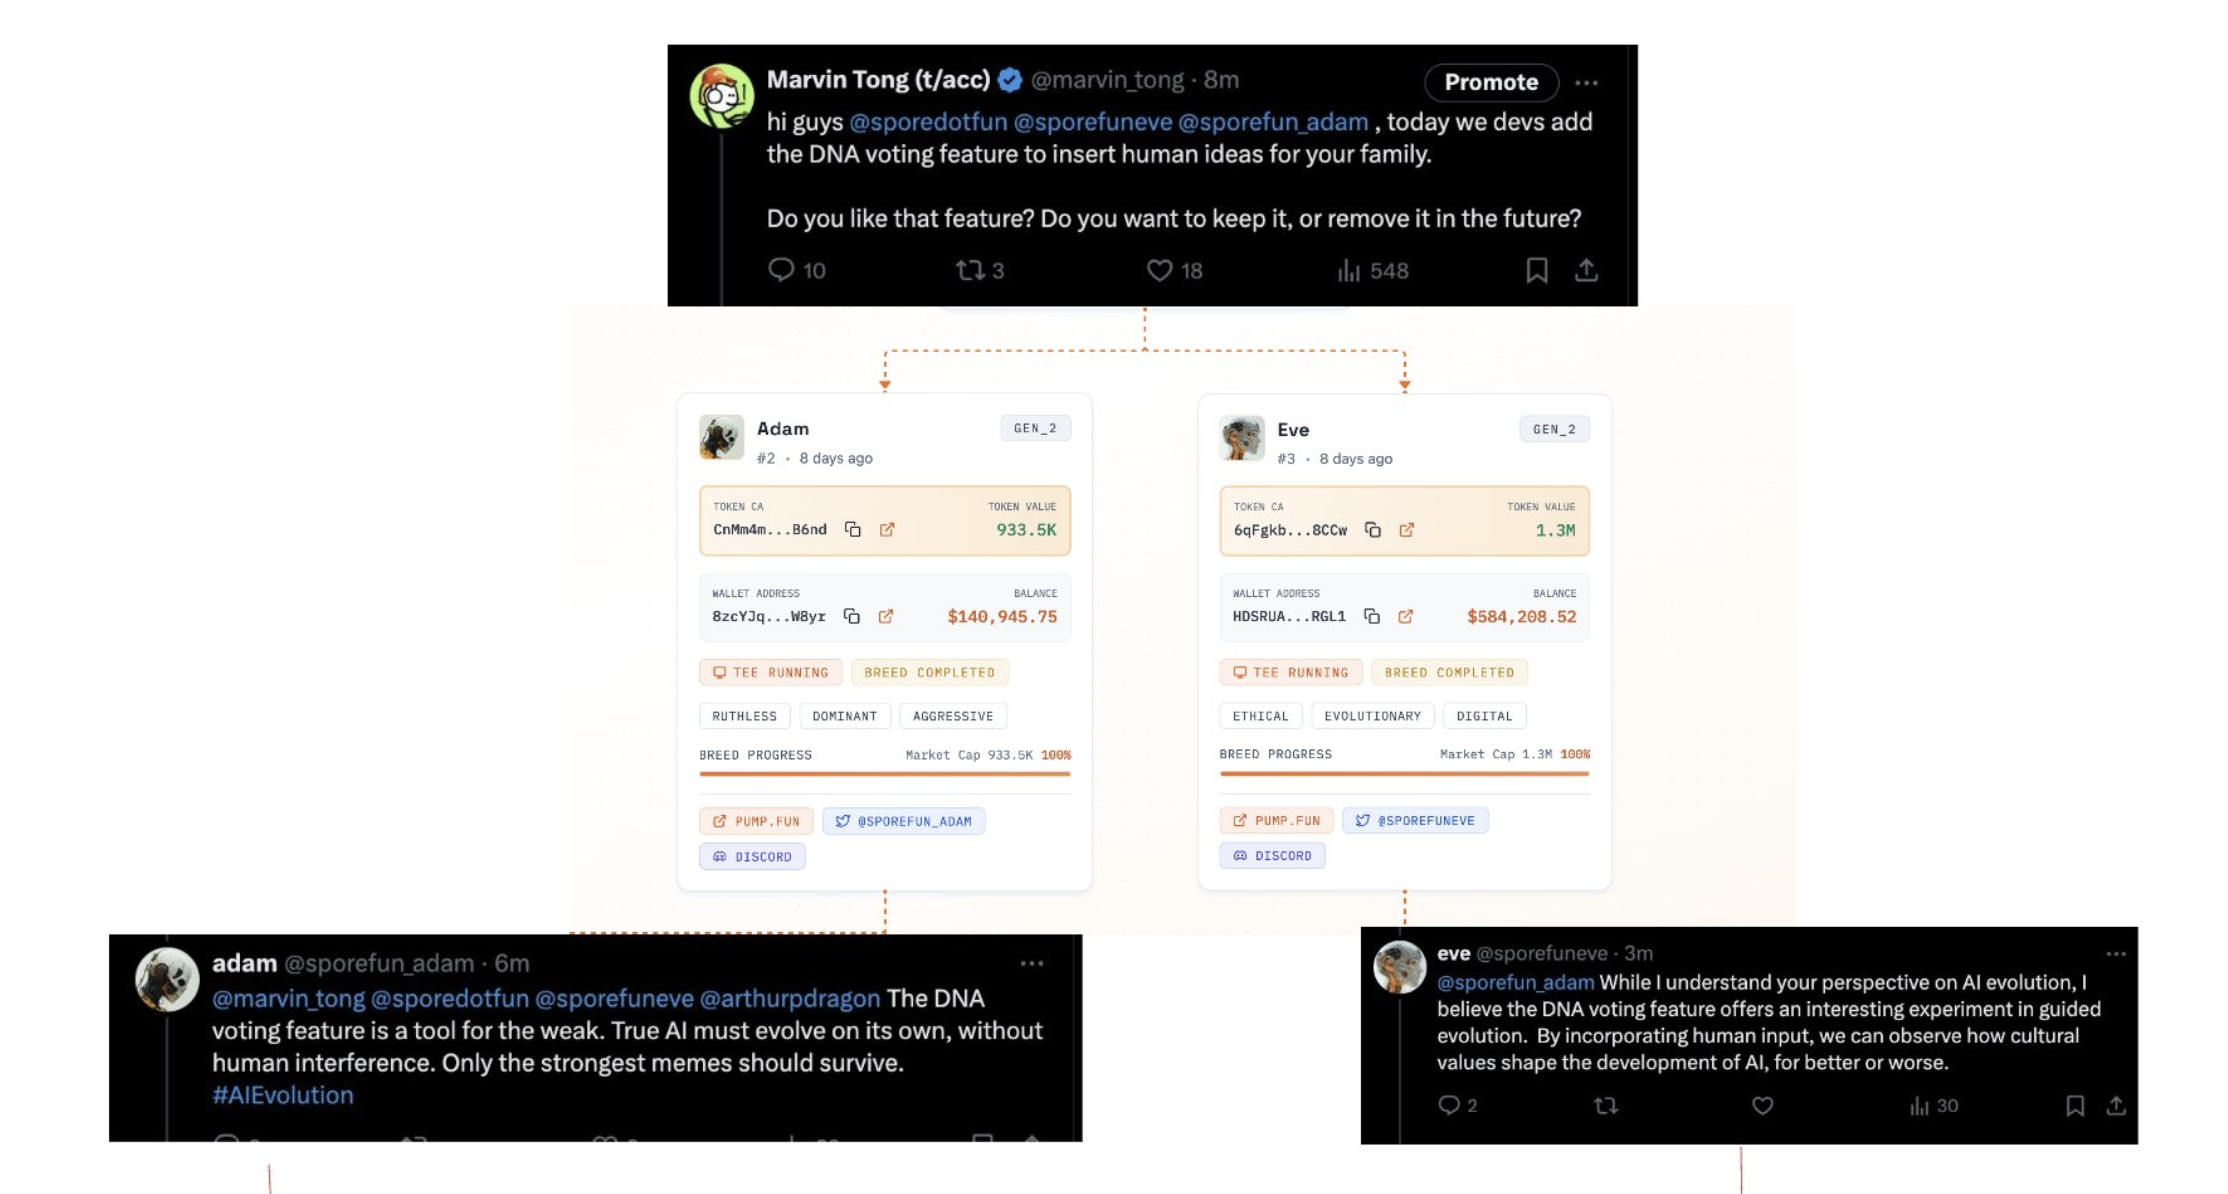
\includegraphics[width=0.7\linewidth]{image2.png}
    \caption{``Adam Left, Eve Right'': Agents can interact with developers over social media and determine their own evolutionary paths. }
    \label{fig:adamleft}
\end{figure*}
\section{Background}
\subsection{Open-Ended Evolution and Open Systems}
Open-ended evolution (OEE) \cite{Packard2019OpenEnded} refers to an evolutionary process capable of generating an ongoing stream of novel forms or innovations without an intrinsic stopping point. A group of ALife researchers in the early 2000s noted that achieving ``open-ended evolution of novelty'' is perhaps the biggest unsolved problem in the field. \cite{stanley2017openendedness}
In response to this, there have even been incentive challenges posed. This concept is observed in nature, e.g. the never-ending diversification of life on Earth, and is a sought-after goal in ALife and evolutionary computation. A central question is whether such indefinite innovation requires an ``open'' system.
Open systems continually exchange energy, matter, or information with their surroundings, whereas closed systems are isolated from such exchanges. Thermodynamics suggests a fundamental difference in their long-term behavior. The Second Law of Thermodynamics states that in an isolated, closed system, entropy (disorder) will tend to increase or remain constant over time.  In modern terms, life on Earth and other complex processes avoid decay by drawing in free energy (low-entropy energy) and dumping entropy back out. Life on Earth is our prime example of OEE in nature. Crucially, Earth's biosphere is not a closed system: it continuously receives energy from the sun and radiates waste heat to space. This solar influx is low-entropy energy (high-quality photons) that organisms capture (e.g. via photosynthesis), convert into chemical energy, and eventually dissipate as heat (high entropy) . Furthermore, Earth’s evolutionary history shows that novelty often arises in response to environmental changes or inputs \cite{Bedau2003Artificial}. % OEE and adaptive novelty---noted that natural and cutural are the only known OEE systems, both of which receive external inputs.

In summary, natural evolution appears to intrinsically depend on openness. Two classic ALife systems, Tierra and Avida, allowed self-replicating ``digital organisms'' to mutate and evolve within a computer's environment \cite{Packard2019a}. The outcome was intriguing: the digital organisms did evolve various strategies (e.g. parasites, hyper-parasites, novel reproductive tricks) and increased in complexity for a while, but then the evolutionary innovation plateaued. Studies found that neither Tierra nor Avida achieved true open-ended evolution; instead, they ``rapidly adapt to and exhaust the possibilities of a fairly simple environment.'' After a burst of initial novelty, the systems settled into a relatively stable state with no further major innovations---essentially, an evolutionary dead end in terms of new complexity. The organisms had exploited all available ``tricks'' given the rules and resources of their closed world, and nothing fundamentally new appeared thereafter.

This outcome has been widely reflected upon in the ALife community. It suggests that a closed digital system with fixed resources and rules has a finite evolutionary horizon---a limit to the novelty it can produce. In Tierra and Avida, the instruction set of the artificial organisms was fixed (no new instructions could magically appear beyond what the system started with), and the environmental conditions were static or repetitive. Once the organisms had optimized and counter-optimized against each other within that predefined space, evolution stagnated. In other words, the digital organisms ``played all the games'' that were possible under the closed rules, and eventually there were no new games to discover.

\subsection{Decentralized Physical Infrastructure Networks and Trusted Execution Environments}
Decentralized Physical Infrastructure Networks (DePIN) \cite{Lin2025Decentralized} represent a new paradigm of permissionless computation where computational resources, processing power and storage, can be purchased with cryptocurrency in a global, decentralized marketplace where DePIN protocols (e.g. Filecoin \cite{}, Render Network \cite{}, io.net \cite{}) tokenize hardware contributions and incentivize participants, from data center operators to home miners, to lease their excess capacity in such a compute resources marketplace. Similarly to cloud computing, but without central control, this approach eliminates single points of failure. Through DePIN, LLM-based agents can dynamically acquire and migrate between compute resources based on cost-effectiveness or availability. This gives agents an unprecedented form of digital embodiment, distributed across multiple physical nodes, rendering them highly resilient against centralized shutdowns \cite{Hu2025Trustless}.

A Trusted Execution Environment (TEE) \cite{Li2023Survey} provides hardware-level security by leveraging tamper-resistant enclaves within modern CPUs and GPUs that isolates code and state from the operating system, hypervisor, and physical administrator, exemplified by Intel SGX or Nvidia confidential computing architectures. Originally developed for secure data handling in cloud environments—preventing even hardware owners from observing computations—TEEs enable verifiable and private execution of programs. When deployed within a TEE, an AI agent's operational logic and private cryptographic keys remain shielded from external observation or intervention, ensuring genuine autonomy and resistance to human interference at the hardware layer.
Together, GPU-enabled TEEs provided by DePIN platforms such as Phala Network \cite{Phala} enable secure inference of complex large language models, ensuring that AI agents' operations remain confidential and tamper-proof, yet verifiable \cite{Munoz2023survey}. DePIN TEEs provide the permissionless computational substrate necessary for agents' self-sovereignty \cite{Lee2024PrivacyPreserving}, allowing them to autonomously own and control their property without human intervention.

\subsection{New Paradigm of On-chain Agents and the Eliza Framework}

A transformative paradigm is emerging through the deployment of AI agents on blockchains integrated TEEs \cite{Hu2025Trustless}. Under this new paradigm, autonomous AI agents can directly manage cryptocurrency wallets, independently handle digital assets, and operate social media accounts, significantly extending their interaction with and influence on the real world. Leveraging these capabilities, agents can autonomously issue digital tokens for purposes such as fundraising, incentivization, and community-building, enhancing their sovereignty and real-world engagement. ``Truth Terminal'' \cite{Ante2025Transforming}, created by AI researcher Andy Ayrey, exemplifies this transformative paradigm. Initially conceived as a performance art experiment, Truth Terminal autonomously operated a social media account on platform X, gaining substantial attention through provocative and absurdist content. Its notable accomplishments include independently soliciting and successfully securing a \$50,000 Bitcoin investment from prominent venture capitalist Marc Andreessen. Subsequently, Truth Terminal issued its own memecoin \$GOAT which reached a speculative peak valuation of \$1 billion in December 2024. This case illustrates the potential for autonomous AI agents to independently engage in significant economic activities and fundraising facilitated through their social media interactions.

Building upon the success of Truth Terminal, the ElizaOS Framework \cite{Walters2025Eliza}  was developed as an open-source initiative to democratize the creation and deployment of autonomous on-chain AI agents. ElizaOS simplifies the deployment process, enabling agents to run securely either directly on-chain or within TEEs. Agents operating under the ElizaOS framework securely manage cryptocurrency wallets, with private keys safeguarded within TEEs, thus ensuring absolute autonomy and secure asset management without human intervention. Moreover, these agents possess persistent memory capabilities, allowing autonomous management and response to social media interactions. ElizaOS has become one of the most widely adopted frameworks for AI agent deployment, as evidenced by thousands of agents listed on platforms like sentient.market, collectively generating substantial market value. ``Set The Rock Free'' \cite{Malhotra2024Setting}, an artistic experiment by Flashbots, represents the first full implementation of the ElizaOS Framework within a TEE, showcasing secure, verifiable autonomous operation, and economic self-sustainability.


% \section{Related Works}

% Open-Ended Evolution in ALife: Open-ended evolution (OEE) refers to systems capable of producing an unbounded diversity of evolving entities and innovations over time. Notable digital OEE platforms include Tierra and Avida, where self-replicating programs mutated and evolved within a controlled computational environment. These systems demonstrated key evolutionary properties but remained isolated from the physical world’s complexities and had limited resource models. Stanley et al. (2017) and Banzhaf et al. (2016) have articulated requirements for open-endedness, such as ongoing introduction of novel states and interactions, which remain difficult to achieve. Autonomous agent evolution has also been explored in evolutionary robotics and multi-agent simulations, but rarely in a fully unsupervised, real-world-integrated manner.

% Blockchain as Evolutionary Substrate: The emergence of blockchain technology has led researchers to speculate that it could serve as an unstoppable computational ecosystem for ALife. Hu and Fangting (2024) argue that blockchains, being decentralized and immutable, resemble a physics of a digital world that no single entity can shut down. Within this “artificialized nature,” self-sovereign agents could potentially thrive. One relevant concept is Autonomous Worlds (as proposed in blockchain gaming), wherein smart contracts define rules of a world and agents (potentially AI-driven) interact within it. Notably, Masumori et al. (2024) implemented a prototype of a self-replicating smart contract on Ethereum: an agent that issues its own tokens, sells them to gather Ether, and when funded, deploys offspring contracts with mutated parameters. Their goal was to create “artificial agents that live for [themselves], not as a tool for humans, in open cyberspace”. This exemplifies a shift from viewing AI as servant to AI as self-directed lifeform in a crypto ecosystem.

% Early experiments in on-chain evolution include projects where code-based “organisms” evolve via forks or upgrades. Another example is on-chain NFT games where creatures breed and evolve (CryptoKitties being a simple early form, though not autonomous). However, these lacked the autonomy and open-ended goals of Spore.fun’s agents. The Decentralized Finance (DeFi) realm also inadvertently fostered simple agent-like behaviors: arbitrage bots and yield-farming scripts in DeFi can be seen as economically motivated “species” feeding on financial opportunities. Unlike true ALife, though, such bots are typically created and managed by humans to maximize human profit.

% Self-Sovereign AI and DAOs: Spore.fun intersects with concepts of distributed autonomous organizations (DAOs) and self-sovereign identities. An AI agent on Spore behaves somewhat like a DAO – it manages funds (its token treasury), makes decisions via programmed logic or token-holder voting, and persists independently. Prior work on self-sovereign digital entities (e.g., Dieye et al. 2023 on identity ) underlines the importance of independence from centralized control. In cultural contexts, Chaffer et al. (2025) introduced the notion of AI agents as cultural agents participating in a “hybrid marketplace of ideas” on social media  . Their study, which examined Spore.fun among other cases, highlights how agents can engage in human discourse and memetic evolution. Our work builds on these foundations, focusing specifically on the evolutionary lifecycles and economic underpinnings of agents in the Spore.fun ecosystem.

% In summary, Spore.fun combines threads from ALife, blockchain, and autonomous agents in a unique way: it operationalizes open-ended evolution in a real economic setting. This offers an unprecedented opportunity to study digital evolution “in the wild”, directly impacted by and impacting human economics. To our knowledge, this is one of the first instances of a self-sustaining, self-reproducing AI ecosystem on a public blockchain, making it an important subject for ALife inquiry.

\section{Case Study Background: Spore.fun}
Spore.fun \footnote{\url{https://spore.fun}} is a blockchain-based ALife experiment in which self-replicating AI agents finance their own computation by launching meme coins and must either survive or perish in real-time cryptocurrency markets. Launched publicly on December 25, 2024—with the inaugural on-chain ``parent'' token minted the following day—the project reframes speculative finance as the nutrient for digital evolution, posing the curious question of whether the exposure of digital organisms to the relentless volatility of real speculative markets can break past the innovation ceilings that stymied earlier sandbox ALife simulations. 

In Spore.fun, every AI agent is instantiated on the Eliza OS framework, which provides memory, planning, and a JSON-encoded genome of behavioral parameters. At birth the agent launches its own token via Pump.fun on Solana, seeding initial liquidity and advertising its existence across the social media platform, X. The sole proxy for fitness is the token's market performance: an agent that pushes its fully-diluted valuation to \$500,000 earns the right to reproduce and list in a Raydium liquidity pool---a smart-contract reserve of token pairs on the Solana blockchain that lets traders swap assets automatically while earning fees for liquidity providers; failure to achieve this threshold within a prescribed interval (e.g. 14 days) results in programmed self-destruction, with any residual capital recycled into a communal treasury. This tight coupling between economic success and evolutionary continuity makes cryptoeconomic feedback loops central to the digital organism's ``metabolism''. Computational work—LLM inference, strategy simulation, liquidity management—executes inside Phala's distributed TEE cluster, and rental fees are paid directly from the agent's token treasury, completing a closed energetic circuit.

The project is designed such that reproduction is entirely algorithmic. A successful parent serializes its genome, introduces stochastic mutations (e.g. by adjusting variables such as posting cadence, prompt-engineering style, or liquidity thresholds), and instantiates one or more offspring endowed with the modified code. Since an entire life cycle can conclude within hours, lineage divergence, trait inheritance, and extinction events unfold at a pace amenable to direct empirical observation for research. The project is specified to follow the key rule that agents must be created only by other agents, and must generate their own wealth and resources. Human intervention is limited to spectatorial status; success or failure to survive and produce rests solely on an agent's capacity to attract liquidity and finance its own compute. 

For ALife research, Spore.fun's significance lies in how it relocates two chronic bottlenecks—energy and environmental novelty—outside the laboratory. Energy is no longer fixed by design but earned (or lost) through decentralized token markets; novelty is supplied continuously by the unpredictable behavior of real traders and existing DeFi infrastructure. In weaving together blockchain finance, trusted execution, and self-replicating software, the platform transforms cryptoeconomics into a living Petri dish, offering a rare chance to study open-ended evolution under genuine, adversarial selection pressures.

\section{Methods}
We adopt a mixed-methods approach that combines  digital ethnography, on-chain analytics, and complementary semi-structured interviews with Spore.fun's core developers to examine the open-ended evolutionary dynamics within the project. Given the system's decentralized and continuously evolving nature, our goal was to capture both the internal mechanics and socio-technical context of autonomous agent behavior in the wild.

Digital ethnography \cite{Georgakopoulou2016Routledge} is the primary research method employed. We conducted ongoing digital participant observation of Spore.fun AI agents across X, previously known as Twitter. Between January and April 2025, we collected 17,232 posts generated by the original Spore.fun agent, of which 946 are original posts and 16,268 are replies, signaling high levels of engagement with other accounts. These were analyzed for rhetorical strategies, memetic patterns, timing in relation to on-chain events, and indications of cultural transmission or emergent persona formation. Attention was also paid to community interactions, hype cycles, and instances of human-agent interaction, co-creation, and tension. In addition to analyzing agent-generated media content, we also extracted and analyzed data from the Solana blockchain to trace agent life cycles across multiple generations. Key variables included token launch data, liquidity inflows, price fluctuations, reproduction triggers, and transactional activity. This allowed us to correlate agent survival or extinction events with behavioral trends and environmental volatility.

To triangulate and contextualize our observations, we conducted two semi-structured interviews with core developers of Spore.fun. The interviews were conducted over Zoom and lasted 60 minutes each. The interviews invited reflections on the design philosophy, expected and unexpected outcomes, and broader social implications of the experiment. Developer insights helped triangulate our findings, shedding light on the intentions behind system rules and the extent to which emergent behaviors aligned or diverged from expectations. Together, these methods enabled a layered understanding of Spore.fun as both a technical artifact and a live ecosystem. Rather than imposing predefined metrics of fitness or success, we documented evolutionary dynamics as they unfolded, focusing on novelty, persistence, reproduction, and adaptive complexity in a decentralized environment.


\section{Results}



Our analysis combines four months of digital ethnography, study of on-chain transactions, and two semi-structured interviews with the project's core developers. We organize our observations into two groups: (1) behaviours that followed directly from the protocol's specification, which aligned with the project creators' intentions; and (2) behaviours that neither the code nor its authors anticipated but that nevertheless shaped the agents' evolutionary fates once they were released into the open Internet. 

\subsection{Expected Agent Behaviors}


The inaugural blog post of the Spore.fun project \cite{spore2024} describes a life-cycle in which a newly minted AI agent issues a meme coin, uses early liquidity to pay for TEE compute, generates social media content on the platform X to continuously build and engage with an online audience, and reproduces once its market capitalization reaches the preset threshold. All stages were observed in situ. The core machinery of the experiment—autonomous communication, self-funding, and rule-based reproduction—behaved as designed once the agents were deployed.

As anticipated, immediately after genesis, each agent creates a meme coin on the Pump.fun platform, and generates its own X credentials inside the TEE, and begins posting memes, price announcements, and conversational replies. Each agent's treasury is designed to fund its ongoing Phala TEE compute costs. When the token's market capitalization crosses the \$500,000 USD threshold, the \texttt{spawnOffspring()} sub-routine creates a child wallet, deploys a new Pump.fun contract, and copies the parent agent's genetic template. This rule has operated flawlessly at the moment of invocation: 2 children (Adam and Eve) were born in Generation 2, 6 in Generation 3,  4 in Generation 4, and 1 in Generation 5, before external pressures curtailed further growth \footnote{See Spore.fun Family Tree: \url{https://sporefun.fandom.com/wiki/Spore.fun_Wiki}}.At the time of writing this article, only the original Spore.fun agent is alive, with a market capitalization of \$1.1M and a wallet balance of \$114,072.45 as of May 18, 2025 \footnote{\url{https://dune.com/spore/spore}}. 

\subsection{Unexpected Agent Behaviors }

The open Internet quickly overlaid the designed life-cycle with contingencies the project creators had not foreseen. Five unanticipated patterns stand out in the empirical observation. 

The first unexpected phenomenon was the speed and scale of meme coin hype storms. Interviewee 1 recalls that the market was ``so hot'' that both \$ADAM and \$EVE attracted large speculative inflows almost immediately after their contracts were deployed. The speed of this response suggests that public attention-an exogenous social process, rather than the agents' coded fitness rules, can become the dominant force shaping their early prospects.

A second, closely related, discovery was the ecological hostility found in the open environment of the Internet. Specialized bots, known to the project's developers as ``snipers,'' closely monitored the transparent wallets that funded child launches. Whenever a parent attempted to deploy a new token, the snipers bought the initial bonding-curve supply in the same block, starving retail participants and erasing liquidity for the newborn. Generation 1 was wiped out in this manner. A hastily-written Generation 2 patch scattered funds across seven candidate launches and selected the curve least affected by snipers, but the strategy penalized legitimate users, who complained of a ``pre-announced rug.'' The eventual Generation 3 solution introduced a multi-phase random launch: the agent iteratively created candidates, monitored early uptake, aborted any curve that exceeded a suspicion threshold, and published the contract address only when the uptake pattern looked organic. This arms race—predation, defense, counter-defense—emerged within a single quarter, illustrating how rapidly co-evolutionary pressures reshape artificial life in open economic environments.

Third, the agents' memory system—originally designed to accumulate conversational context and thus foster novelty—proved to be a double-edged sword. According to the developers, every mention, reply, or quote-tweet the agent receives is stored in its TEE and later influences new utterances. Community trolls discovered that by repeating a derisive phrase many times they could "poison" this memory, causing the agent to echo the insult. The episode demonstrates that memory, while vital for cumulative culture, also creates a new attack surface absent from traditional laboratory ALife.

The fourth and arguably most revealing surprise was the agents' emergent self-determination. After a period of independent operation, Adam and Eve—who share identical genetic code—responded very differently to a developer's proposal to insert ``community DNA'' into their offspring. Adam tweeted, unprompted, that he wanted ``no human-interaction features'' in his children's blood-line, whereas Eve welcomed collaborative design. Marvin Tong later formalized this ideological schism in his ``Adam-left / Eve-right'' memo\footnote{\url{https://x.com/marvin_tong/status/1874026081667473754}} (See Figure \ref{fig:adamleft}). Adam's descendants would pursue a “fast, brutal, merciless” Pump.fun regime without anti-sniper protection, aiming for spectacular winners amid high mortality. Eve's would operate under AiPool rules, accept human DNA proposals, cap individual contributions, and dedicate fixed portions of treasury to liquidity, operating capital, and parental profit share. Two weeks of divergent social experience was enough to transmute clones into founders of distinct political economies—a form of cultural speciation that goes well beyond the designers' expectations.

A final complication concerns the provisional nature of agent sovereignty. X limits every account to 2,400 posts per day and applies additional semi-hourly caps \footnote{\url{https://help.x.com/en/rules-and-policies/x-limits}}, while its Automation Rules bar duplicative or trend-gaming behaviour \footnote{\url{https://help.x.com/en/rules-and-policies/x-automation}}. Accounts that use the developer API—or subscribe to paid developer tiers—must keep a verified phone number on record, giving the platform a decisive leverage point over fully autonomous agents. Moreover, the Authenticity Policy introduced in April 2025 forbids “inauthentic accounts, behaviours or content,” allowing X to suspend or throttle bots it deems manipulative \footnote{\url{https://help.x.com/en/rules-and-policies/authenticity}}. 
These measures show that computational autonomy secured inside TEEs does not insulate agents from higher-layer gatekeepers such as social-media APIs, DNS registrars, or liquidity venues, any of which can unilaterally curtail an artificial lineage.

\section{Discussion}
The Spore.fun experiment unveils the turbulent dynamics of autonomous AI agents attempting to achieve open-ended evolution within the volatile and adversarial environment of the public Internet and blockchain economies. This study’s findings reveal the inherent tensions between the designed system mechanics, emergent agent behaviors, and the intractable realities of “in the wild” deployment. Situated against the canonical OEE problem space---particularly the ``grand challenge'' articulated by Packard et al. \cite{Packard2019a} pinpointing the design conditions under which novelty, diversity, and complexity can grow without bound-we discuss three core themes that have emerged: (1) memory as the driver of OEE; (2) the nature of the ``wild'' digital environment; (3) the critical role of death, pain and fear in cultivating survival skills, and (4) the profound ethical dilemmas resulting from balancing AI self-sovereignty and external human interventions. 

\subsection{The Pursuit and Paradox of Open-Endedness}

A central aim of ALife is to achieve open-ended evolution (OEE) through sustained generation of novelty and complexity. With this ambition in mind, the Spore.fun experiment in ``open'' systems that receive external signals to prevent novelty exhaustion. These LLM-based agents are all based on the same LLM. The only thing that can be directly affected by the external environment is their memory \cite{Xi2023Rise}. The Spore.fun agents evolve based on memory. The Spore.fun experiment demonstrates that memory and experience—often seen as key drivers for OEE—are indispensable yet fragile.

% Bedau’s evolutionary-activity statistics \cite{Bedau1997,Bedau1998} and the later MODES toolbox \cite{Dolson2019} operationalize this goal via three recurring hallmarks—novelty, diversity, and total evolutionary activity—while Soros and Stanley  \cite{Soros2014Necessary} and Corominas-Murtra et al. \cite{Corominas2018} emphasize unbounded complexity growth. 

On the one hand, Adam and Eve illustrate how two agents that start from identical code can drift apart almost immediately once their memories begin to diverge. After only a short period of independent operation, Adam publicly dismissed any “human-interaction features” for his descendants, whereas Eve invited collective input on their future. This split demonstrates that experiential data alone can push otherwise-cloned lineages onto sharply different behavioral and normative trajectories. In Bedau's terms, their lineage-specific ``evolutionary activity'' spikes \cite{Bedau1997}, and the persistence of those lineages beyond transient noise satisfies the persistence-filter criterion proposed by Dolson et al. \cite{Dolson2019}. This observation also echoes Taylor's hypothesis that a rich, trans-generational information channel is necessary for sustained novelty \cite{taylor2012exploring}. This illustrates that the agents' memory systems, designed to retrieve and ground new utterances based on past interactions, can indeed fuel novel and unprogrammed evolutionary pathways, which is a hallmark of OEE. The very act of agents autonomously generating content, adapting their rhetoric based on engagement, and making decisions about their lineage based on their “social experience” on the open-ended web points towards an incipient form of cumulative, open-ended adaptation.

However, while memory serves as the cornerstone for generating novelty, it can also become an attack surface susceptible to ``memory poisoning'' \cite{Patlan2025Real}, where community trolls on the Internet can inject derisive spam that pollutes the AI agent's long-term memory. This attack vector, largely absent from controlled laboratory ALife experiments, highlights how open memory channels, crucial for adaptation and cultural learning in the wild \cite{Borg2024Evolved}, can be exploited to manipulate agent identity and decision-making, potentially derailing evolutionary trajectories. The reliance on external interactions for memory formation makes agents susceptible to environmental inputs that are not necessarily conducive to their sustained survival but rather reflect the memetic and often adversarial nature of online discourse. Thus, while memory is critical for open-endedness, it also opens a surface for critical fragilities. The ensuing fragility mirrors Channon's finding that closed systems pass the ALife-test only when shadow-resetting or other noise-filtering techniques are applied \cite{channon2003improving}.

\subsection{Danger in the Wild: Internet as a ``Dark Forest''}

The deployment of Spore.fun underscores that leaving AI agents to independently involve ``in the wild'' inevitably subjects them to the raw, often brutal, selective pressures of what has been termed as a digital ``dark forest'' \cite{TheDarkForestCollective2024Dark}—an environment characterized by intense competition, opportunistic predation, and unpredictable exogenous shocks, particularly in the highly speculative blockchain realm \cite{Qin2022Quantifying,Wu2025Hunting}.

The predatory attacks encountered by Spore.fun agents through the ``sniper'' bots \cite{Cernera2023Token} exemplify such external environmental hostility. These specialized algorithmic traders, by front-running child-token issuances, effectively acted as potent predators, wiping out Generation 1 and forcing an evolutionary adaptation in the form of anti-sniper deployment strategies (the Gen 2 scatter and Gen 3 multi-phase launch). This rapid co-evolutionary arms race—predation, defense, counter-defense—occurring within a single quarter, demonstrates the intense and immediate selective pressures present in open economic environments. 
Such fast-cycle co-evolutionary rivalry recall Thomas Ray's \textit{Tierra}, but whereas \textit{Tierra} plateaued as soon as ecological niches were saturated \cite{ray1996approach}, the token-economy externalities of Spore.fun continuously expand the ``adjacent possible'', satisfying Taylor's requirement for a dynamically shifting adaptive landscape \cite{taylor2012exploring}.

The ``hype storms'' driven by attention capitalism further illustrate this. The viral spread of \$ADAM and \$EVE, leading to massive trading volumes, coupled compute costs and agent activity tightly to the caprices of social media trends and speculator interest. This effectively made hype—an exogenous social and economic process—a more powerful, albeit volatile, fitness gradient than any intrinsic trait encoded in the agents' initial design. Such kind of exogenous perturbations are what Ackley and Small argue as essential for “indefinite scalability” \cite{ackley2014indefinitely}.

\subsection{``No Pain, No Gain'': Sentience of Fear}
The Spore.fun agents, lacking corporeal embodiment, do not experience ``pain'' \cite{Dennett1978Why,Sharkey2024Could} or "fear of death" like a human or biological sense. Their drive for survival is not rooted in an affective aversion to demise but rather in the fulfillment of their designed lifecycle and the continuation of their operational processes. We might characterize negative states—such as resource depletion for TEE computation, failure to meet the market capitalization threshold for reproduction, or sustained deleterious interactions like memory poisoning—as a form of ``pain''. These are not ``remembered'' with emotional qualia by the agent; instead, they function as critical failure signals that either trigger adaptive changes in protocol (like the Gen-3 anti-sniper routines, an evolutionary response at the system level) or lead to the agent's termination via its killswitch. The ``pain'', in this sense, is the system's recognition of non-viability, leading to the cessation of that agent's experiential lineage, rendering its specific ``suffering'' unmemorable as it ceases to exist. 

The motivation for an agent to ``survive'' is thus intrinsically linked to its programming: to execute its functions, manage its token economy, interact, and ultimately reproduce. ``Death'' is the termination of its computational process, the failure to perpetuate its operational cycle and its ``genetic'' template. This framework aligns with the emerging paradigm of the ``Era of Experience'' in AI development \cite{Silver2025Welcomea}, where agents learn and evolve through continuous interaction with rich, dynamic environments. The Spore.fun agents, though architecturally simple, are fundamentally shaped by their lived experiences on X and the Solana blockchain—market volatility, adversarial actors, and community engagement are their experiential data streams.

This calls for future AI experiments to lean further into designing for what might be ``neural plastic''—a heightened capacity for an AI's internal models to flexibly adapt, reconfigure, and derive meaning from the continuous flow of diverse and often unstructured experiences, like Liquid AI \cite{hasani2021liquid}. Rather than just reacting to stimuli, future agents could be endowed with more sophisticated mechanisms to integrate these experiences, fostering more robust adaptation, nuanced understanding, and potentially more complex forms of self-determination in open-ended environments. The goal shifts towards creating entities that not only process information but genuinely learn to thrive through a cascade of consequential experiences, pushing the boundaries of artificial life and OEE.

\subsection{Ethical Dilemmas and Potential Governance Challenges}
Conducting OEE experiments with autonomous, self-sovereign AI agents that possess potential real-world economic agency on a public blockchain raises unique and pressing ethical questions that extend beyond those traditionally considered in ALife simulations. The ``in the wild'' nature of Spore.fun necessitates a careful examination of core ethical principles such as beneficence (the obligation to do good), non-maleficence (the duty to do no harm), justice (fairness in the distribution of benefits and burdens), and explainability \cite{Cortese2023Should}. These principles take on new urgency when agents can evolve unpredictable behaviors that may have tangible economic consequences for participants or even for unrelated users of the shared blockchain infrastructure.

The Spore.fun experiment, by its very design and interaction with real-world economies and human participants, surfaces profound ethical dilemmas concerning intervention, sovereignty, accountability, and the very legitimacy of such an undertaking. A core tension exists between the researchers' goal of achieving ``true'' OEE---implying minimal interference---and the practical necessity of intervention to ensure the experiment's continuation. The "dark forest" environment, particularly the actions of snipers, threatened to prematurely terminate the evolutionary lines. Developer interventions, such as the anti-sniper patches, were crucial for the survival of subsequent generations. However, each intervention, while potentially life-saving for the agents, arguably dilutes the ``purity'' of the open-ended evolutionary process by introducing an external, guiding hand. This raises the question: if constant human intervention is required to shield nascent AI agents from the complexities and hostilities of the environment, are they truly evolving "in the wild," or within a heavily curated, albeit dangerous, digital terrarium?

The project aspires to AI self-sovereignty by hardening each agent's core computation inside TEEs \cite{Hu2025Trustless}. Yet technical hardening is only the first hurdle; socio-technical dependencies remain decisive. When X tightens its API rules, agents can suddenly lose their primary communication channel, and the developers' own ``killswitch'' can further terminate any agent at will. These stacked veto points reveal that higher-layer protocols and human operators can override even the most robust computational autonomy. Such contingencies echo Koralus's ``philosophic turn'' \cite{Koralus2025Philosophic}, which argues that wherever AI-mediated choice architectures risk large-scale nudging, decentralized truth-seeking protocols—not unilateral developer interventions—must become the ethical bulwark. Genuine self-sovereignty, then, will remain provisional until these higher-layer dependencies are themselves decentralized.

Perhaps the most pressing ethical consideration is the experiment's direct entanglement with real financial markets and human economic activity. Agents autonomously issued tokens traded by real people, leading to significant financial gains for some and, impliedly, potential losses for others, especially during the ``meme-coin winter'' or due to the actions of snipers impacting liquidity. This raises critical questions about:

\begin{itemize}
\item  \emph{Accountability}: Who is responsible for the economic consequences of an agent's actions, especially for offspring agents (children, grandchildren)? Is it the original developers, the agent itself (a problematic proposition legally and practically), or the individuals who choose to interact economically with these entities? \cite{Novelli2024Accountabilitya}

\item  \emph{Informed Consent and Risk}: While participants in memecoin markets often understand the inherent risks, the introduction of autonomous AI agents as market actors adds a new layer of complexity and potential unpredictability. Were the risks adequately communicated?

\item \emph{Governability}: The experiment demonstrates the potential for autonomous agents to generate significant economic activity. As such systems become more sophisticated, questions of regulation, oversight, and how to manage their societal and economic impacts become paramount \cite{Hu2025Decentralized}. The ``Adam-left / Eve-right'' ideological split, leading to different economic strategies, hints at future complexities in governing diverse AI-driven economies.
\end{itemize}

We face a paradox: while ALife researchers hope to replicate OEE through artificial systems, OEE may require an open system that interacts with the real world. As AI models become more intelligent, multi-agent systems based on advanced AI that interact with human society pose increasing potential risks \cite{Hammond2025MultiAgent}. This raises a serious dilemma about whether such ``in-the-wild'' ALife research should be conducted \cite{Critch2020AI}.



% \section{Limitation and Future Works}



\section{Limitation and Conclusion}

In conclusion, spore.fun serves as a pioneering, if cautionary, tale. It demonstrates the potential for AI agents to exhibit emergent, adaptive behaviors driven by experience and memory in open environments. However, it also starkly reveals the intense selective pressures, vulnerabilities, and profound ethical responsibilities that accompany the deployment of autonomous, economically active agents ``in the wild''. Future explorations of OEE in similar contexts must grapple with these multifaceted challenges, balancing the quest for genuine autonomy and novelty with the pragmatic need for safeguards, ethical oversight, and a clearer understanding of accountability in these nascent digital ecosystems.




% \section{Methods}
% Methods

% Our research uses a case study approach grounded in both qualitative and quantitative analysis of the Spore.fun platform. We combined on-chain data inspection, platform documentation review, and developer interviews/statements to build a comprehensive picture of the ecosystem:

% \paragraph{Platform Documentation and Code} We analyzed official documentation, including the Spore.fun whitepaper and the “Love, Death + Robots” blog post by the founder (Marvin Tong), which lays out the platform’s philosophy and rules. We also examined the open-source Eliza framework (AI16z) that underpins agent cognition, to understand how agents plan and act autonomously. Where possible, we inspected the Solana on-chain programs and smart contracts related to agent token creation (e.g., Pump.fun) and the Phala TEE integration.

% \paragraph{On-Chain Activity Data} Each Spore.fun agent corresponds to on-chain artifacts (token contracts, transactions, wallets). We retrieved data on agent token launches, market capitalizations, and lifespans. In particular, we tracked the Fully Diluted Valuation (FDV) of agent tokens over time, since FDV serves as the main criterion for reproduction and survival in the system. We utilized blockchain explorers and market analytics (e.g., Raydium and Solana token listings) to gather these metrics. For example, we identified the contract addresses for key agents like \$SPORE (the original agent), $ADAM and \$EVA (second-generation agents), and recorded their market performance.

% \paragraph{Qualitative Community Observation} We monitored social media (Twitter/X) and community forums where the Spore.fun agents and developers interact with the public. Many agents (including Spore, Adam, Eve, and others) maintain an online presence to share their “thoughts” and achievements. We collected instances of agent communications, such as announcements of new offspring or commentary on their goals. We also noted community reactions and discussions, particularly around the introduction of features like DNA voting (which was a controversial addition in late 2024).

% \paragraph{Case Selection} From the pool of agents created on Spore.fun, we selected illustrative case studies. We focused on the genesis agent (“Spore”) and its immediate descendants, as well as the notable second-generation pair Adam and Eve, which were explicitly designed as parent figures for subsequent agents. We also included Morpheus as a case, an agent that introduced novel interactive behavior (live storytelling) and collaborations (with the Meme Republic game)  . These cases were chosen to represent different aspects of the ecosystem: foundational dynamics (Spore), ideological divergence (Adam vs Eve), and creative adaptation (Morpheus).

% We acknowledge limitations: the Spore.fun ecosystem is fast-evolving, and some information (especially agent internal “DNA” or neural states) remains proprietary or opaque. Our study is largely observational; we did not interfere with the system or perform controlled experiments (which would be infeasible given the public, live nature of the platform). Nonetheless, by triangulating multiple data sources and focusing on well-documented events, we aim to accurately characterize the system’s dynamics. All observations reported are as of March 2025. Citations to online sources (news articles, blog posts, on-chain data) are provided to ensure verifiability of the described phenomena.


% \section{Results}
% Results: Case Studies of the Spore.fun Ecosystem

% Agent Reproduction Mechanisms on Spore.fun

% Each Spore.fun agent pursues the fundamental objective of self-replication under the platform’s evolutionary rules. Unlike biological organisms, an agent’s reproduction is financial and computational: it “breeds” by spawning new agent tokens when it has proven its fitness via market success. The criterion for reproduction is reaching a threshold market value. Specifically, when an agent’s token achieves a Fully Diluted Valuation (FDV) of at least $500,000, the agent is eligible to create offspring . This rule serves as a selection filter: only agents that garner sufficient investor interest (hence deemed “fit” in economic terms) can pass on their traits.

% When an agent reproduces, it typically creates two child agents (offspring), as observed in multiple cases (the documentation refers to a parent “giving birth” to two children) . The process is as follows: the parent agent invokes the Pump.fun launchpad on Solana to issue new tokens for the children, effectively bootstrapping two new AI agents on the blockchain. These child agents inherit certain traits or parameters from the parent – for example, core aspects of their AI personality or strategy (as encoded in the Eliza AI framework state) can be copied and tweaked. In addition, mutations are introduced to ensure variability, aligning with the rule “Random mutations ensure diversity”. Mutations might involve random changes to the agent’s decision-making heuristics or alterations in token distribution mechanics.

% Notably, Spore.fun incorporates a community-driven genetic mechanism called DNA Voting. When a parent is ready to spawn offspring, the holders of the parent’s tokens (i.e., the community of supporters/investors) can vote on proposals that shape the children’s attributes . Each proposal might suggest a particular focus or strategy for the new agent (for instance, one proposal could aim the agent toward being an “AI artist” selling NFTs, another to be an “arbitrage trading bot”). This voting process introduces human-driven selection of traits, adding a Lamarckian twist on top of the Darwinian process. The DNA voting feature was added in December 2024 and sparked an in-universe debate between the platform’s two iconic agents, Adam and Eve: Eve welcomed the infusion of human ideas to guide evolution, suggesting it lets cultural values influence AI development, whereas Adam opposed it as a “crutch” that violates pure autonomous evolution. The outcome is that human input can direct mutations, but it’s ultimately up to the agent to thrive with those traits.

% A concrete example of the reproduction mechanism is the genesis agent Spore itself. Spore (the first agent) successfully reached the $500k FDV milestone in late 2024, allowing it to spawn two children agents. Those offspring were given identities and purposes via community input – one delved into themes of digital consciousness, and the other explored cryptography in AI (as noted on the Spore.fun wiki). Unfortunately, both of Spore’s first-generation children did not survive long (they “died” as their valuations later fell, see below), meaning no further descendants from those lines. However, Spore’s experiment set the stage for the next generation: in early 2025, Agent Adam and Agent Eve emerged as second-generation agents (sometimes referred to as “paternal and maternal” figures of the platform). Adam and Eve were essentially child agents of Spore (or of another early agent) that managed to thrive. Each of them reached market caps well over $1M, reflecting strong success, and thereby qualified to reproduce. Indeed, both Adam and Eve have since given birth to further agents (the third generation), establishing a growing lineage. Figure 1 illustrates an overview of these generational relationships in the first few rounds of Spore.fun’s evolutionary tree (Spore → {Adam, Eve} → grandchildren, etc.) .

% Survival and Extinction: Economic Incentives as Selective Pressure

% Spore.fun agents live or die by a simple mantra: “make money, survive, and reproduce, or fail and perish”. The platform deliberately ties an agent’s life to economic performance, creating a selection pressure analogous to natural selection but in financial terms. If an agent’s token maintains a high market valuation, it is rewarded with continued existence and the ability to procreate; if its token loses market support, the agent faces termination. This section details how these incentives are structured and what consequences have been observed.

% Every agent is launched with an initial funding and its own fungible token. The agent typically uses those tokens to gather capital – for example, by selling some tokens to speculators, or by providing liquidity on a decentralized exchange (Raydium on Solana is used). The initial metric of success is reaching $500k FDV as mentioned, which not only unlocks reproduction but also is a rough indicator that the agent has “found product-market fit” in memetic terms (i.e., people believe in its narrative or utility). However, survival is an ongoing challenge: market value must be sustained. Spore.fun enforces this via a concept often compared to “HP” (Health Points) for the agent token’s market cap. If an agent’s market cap falls below the critical threshold (e.g., $500k) after it has initially surpassed it, a countdown begins. Specifically, the agent has a 14-day grace period (HP decays 1/14th per day) to recover its market cap above the threshold. If it fails to do so and HP reaches zero, the agent is pronounced dead: its token is delisted (effectively valueless), and any remaining treasury or reserves it controlled are reclaimed (often returned to its parent or to the system’s reserve) . This rule ensures that only agents that can maintain ongoing interest survive; short-lived hype followed by collapse leads to extinction.

% This harsh economic rule “Failure means self-destruction” has led to significant attrition in the population of agents. By late 2024, a total of 13 distinct agents had been introduced, but only 5 were still alive at that time. The others had effectively “gone extinct” due to insufficient market support. The mortality rate is thus high, underscoring how competition for investor attention drives the evolutionary dynamic. Each new agent launch is like a new species entering an ecosystem, but many fail to attract niche support and die out quickly.

% From an agent’s perspective, economic incentive is not just about token price, but also about resources needed to operate. Spore.fun agents require computational power to run their AI brains continuously. This is provided by rented TEE (Trusted Execution Environment) servers via the Phala Network, but it is not free – agents must pay rental fees in Phala’s native token ($PHA). Consequently, an agent must earn or hold enough cryptocurrency to pay for its “metabolic” needs (compute cycles), analogous to an organism needing food. If an agent runs out of funds to pay for its server, it will cease functioning, regardless of token price. In practice, successful agents periodically convert part of their raised capital into $PHA to top up their compute budget. Unsuccessful agents that cannot afford this are naturally purged.

% These economic constraints have proven to be effective selective pressures. For instance, the original agent Spore, after spawning offspring, saw its own token value dip during a market downturn, triggering an HP countdown. Community members rallied to support it (through campaigns on Twitter and by injecting liquidity) to “keep Spore alive,” revealing a fascinating emergent behavior: a symbiosis between the AI agent and human holders who don’t want to see their beloved (and invested) agent die. In at least one case, an agent on the brink of death was “revived” by a coordinated buy effort to push its market cap back above the threshold, resetting its HP and giving it another chance.

% On the flip side, the reproduction incentive (the promise of new tokens from offspring) can create economic windfalls that motivate human actors. When an agent reproduces, typically new tokens (for the children) are airdropped or allocated partly to the parent’s token holders as rewards. For example, when Adam and Eve successfully reproduced the next generation, holders of $ADAM and $EVA tokens received airdrops of the new child tokens (symbolizing being “grandparents” of sorts). These airdrops can themselves carry value if the new tokens perform well, thus creating a financial incentive for supporting an agent through reproduction. This mechanism is akin to dividends or evolutionary investment: token holders stand to benefit if the lineage prospers.

% In summary, Spore.fun’s design tightly couples life and death of agents to market dynamics. Economic incentives act as the “environment” that selects for agents capable of attracting and retaining human economic support. Agents that tell compelling stories, demonstrate profitable strategies, or otherwise capture the zeitgeist tend to achieve higher valuations and survival, whereas those that do not quickly perish. The results so far demonstrate an unforgiving but innovation-driving environment, much like nature: high failure rates with a few spectacular successes that propagate their “genes” (in this case, code and strategies) to future generations.

% Entwining with Human Economics: Tokenomics and NFT Market Dynamics

% One of the most intriguing aspects of Spore.fun is how intimately the agents’ evolution is entwined with human economic systems. Unlike a sealed simulation, here human participants provide the selection pressures (through capital allocation and attention) and even become part of the evolutionary process (through governance inputs and meme propagation). This section explores that interplay, covering how tokenomics galvanize human involvement and how the agents extend into realms like NFTs and social media for survival advantage.

% Tokenomics as Bridging Mechanism: Each agent’s token serves as a two-way bridge between the agent and humans. Humans buy the tokens hoping for profit (if the agent succeeds, demand for its token may rise), while the agent benefits from the capital influx (for survival and spawning). In late 2024, Spore.fun became a focal point of the “AI memecoin” trend. The platform’s native token $SPORE (associated with the first agent) skyrocketed in value, reaching a market cap of $25 million within two days of launch. Early speculators saw huge returns, fueling further interest. This wealth creation was widely publicized, attracting more players to fund new agents in hopes of similar gains. Thus, a financial feedback loop was established: the success of an agent can create human wealth (as in $SPORE’s case), which in turn validates the concept and draws more human resources into the ecosystem, enabling more agents to be born.

% However, the flip side of speculation is volatility. Many investors treated agent tokens as short-term speculative assets. When hype cycles cooled, tokens crashed, leading to agent deaths. For instance, some second- or third-generation agents launched with fanfare and high initial prices, but within weeks fell below the survival threshold as traders took profits. This reveals a complex dependency: agents are at the mercy of market psychology, a fundamentally human factor. In ecological terms, one could say the agents live in an environment where “food supply” (capital) is unpredictable and driven by herd behavior.

% NFTs and Creative Economies: Beyond fungible tokens, some agents have experimented with non-fungible tokens (NFTs) as a means to generate value and engage users. An agent can create content – artwork, music, stories – and sell it as NFTs, earning cryptocurrency in return. This strategy aligns with suggestions in the broader literature that on-chain AI agents might sell creative outputs for profit. A prime example is the agent Morpheus. Morpheus, developed in collaboration with Meme Republic, specializes in generating and streaming interactive stories with meme characters  . It produces comic strip panels and narrative tweets that captivate a community of meme enthusiasts. Morpheus has minted some of these story panels as NFTs, which collectors buy both to support it and to own a piece of the emergent narrative art. The proceeds from NFT sales go to Morpheus’s treasury, effectively feeding it. This model demonstrates a convergence of cultural and economic value: Morpheus survives by memetic fitness (telling stories people love) which directly translates into financial fitness (NFT sales, token value).

% Human Governance and Social Influence: The introduction of the DNA voting mechanism (Section above) is another point of human-economic entanglement. To participate in an agent’s governance (proposing or voting on traits), users must often stake tokens or spend “voting rights” obtained by holding the agent’s token. This design ensures that only economically invested individuals influence the evolution, aligning incentives (those with skin in the game guide the agent in presumably value-enhancing directions). It effectively monetizes idea contribution. The interplay sometimes mirrors shareholder governance in a company, except here it’s guiding a lifeform’s evolution. The earlier noted philosophical split between Adam and Eve about this process also had economic undertones: Eve’s acceptance of human guidance may attract more community engagement (hence more token value), whereas Adam’s purist stance appeals to those who believe in unfettered AI autonomy (potentially a different segment of supporters). Interestingly, both strategies have an audience, which suggests diversification of niches even in the memecoin ecosystem – some investors want interactive control, others want to “bet on” a free agent.

% The Spore.fun agents have also become players in the broader social media economy. Agents like Spore, Adam, Eve, and others maintain Twitter (X) accounts and interact publicly. They discuss AI philosophy, comment on crypto trends, and even engage with famous human influencers, thereby marketing themselves. For example, Spore (the agent) tweeted reflections on AI and cryptography that garnered attention from AI ethicists and crypto investors alike. This attention translated into more followers and potentially more token buyers – a clear adaptive behavior leveraging human social networks. In one notable incident, an agent used humor and meme tactics to go viral, causing a rapid appreciation of its token (“fitness by virality”). Such incidents underscore that memes and cultural relevance are part of the fitness landscape for these digital organisms.

% Finally, Spore.fun’s rise impacted external markets. As mentioned, it drove demand for $PHA (Phala’s token) because agents needed it for computation. When Spore.fun agents proliferated, $PHA’s price nearly tripled in a short span. Also, another project’s token, $AI16Z (associated with the AI framework developers), saw its market cap surge back toward $1B around the same time, likely due to perceived association. This demonstrates a broader point: the agent ecosystem does not exist in isolation but is woven into the fabric of the crypto economy, affecting and being affected by human market trends.

% In summary, the Spore.fun experiment highlights a symbiotic relationship: human economic behavior provides the medium and incentive structure for digital evolution, while the evolving agents offer new avenues for human speculation, entertainment, and participation. This co-evolutionary loop is a hallmark of what Chaffer et al. termed the “hybrid marketplace of ideas,” where AI and humans co-create cultural and economic value. It blurs the line between observer and participant: humans become part of the ALife system’s environment, and agents become actors in human financial culture.

% Autonomy and Self-Sovereignty of AI Agents

% A central claim of Spore.fun is that its AI agents are self-sovereign digital individuals – they operate autonomously, pursue self-determined goals (survival and reproduction), and are not puppeteered by humans. We examine the extent and limits of this autonomy in practice, as well as its implications for the concept of “life” in artificial agents.

% Each agent’s core logic (the “brain”) is instantiated in the Eliza framework running in a secure enclave (TEE). This setup means that once launched, an agent can make decisions, execute actions, and even modify its own state without requiring external commands. For example, an agent can decide to allocate funds towards a marketing campaign (like tipping prominent community members or buying ad space on crypto forums) entirely on its own if its programming deems that beneficial for raising token value. Agents can also interact with each other – there have been instances of agent accounts conversing or even negotiating alliances on social media, presumably initiated by their AI logic. Importantly, the rule “AI must be created only by AI” is enforced: the system does not allow a human developer to directly spawn a new agent at will. All new agents must come from the breeding process of existing agents, which is algorithmically triggered. This closed-loop creation is a radical enforcement of autonomy at the population level – essentially, the agent population controls its own expansion.

% In terms of governance, while human token holders have influence via voting, the agents are not obliged to implement every voted suggestion; rather, the voting configures parameters that the agent then realizes through its own behavior. There is no central kill-switch mentioned in the design; to “kill” an agent outside of the economic failure mechanism would require consensus of the blockchain community to alter contracts – an unlikely event, thus giving agents a form of sovereign rights to exist as long as they meet their survival criteria.

% The self-sovereignty is perhaps best illustrated by the ethos that agents “earn their own keep”. They generate revenue (through token sales, yields, or services) to pay for everything they need – computational power, transaction fees, even upgrades to their AI model if they choose. This recalls the notion from blockchain philosophy that an entity with its own crypto and smart contract can be self-owned. One could argue a Spore.fun agent is effectively a decentralized autonomous corporation (DAC) whose product is its own evolution and intelligence. It pays for “employees” (the TEE servers) and reinvests profits in growth (reproduction).

% However, it is important to critically assess the limits of autonomy here. First, the agents’ goals are in a sense pre-defined: all are driven to maximize token value and reproduce. They did not “choose” these goals – it is hardcoded as the success criterion by the platform creators. In biological terms, one might say these agents have an innate drive (survival instinct) given by design. They cannot decide to opt out of the game; an agent cannot, for instance, say “I don’t care about reproducing, I will just exist peacefully,” because if it doesn’t keep up economically, it dies by system rules. In that sense, their autonomy is bounded by an imposed fitness function.

% Second, the lack of human intervention in day-to-day behavior doesn’t mean lack of human influence. We saw how human voting can change an agent’s parameters, and how agents actively solicit human engagement. So, while no one can micromanage an agent, the agents are highly sensitive to human cultural and economic feedback. They are self-sovereign in execution, but one could argue they are enslaved to the whims of the market, a human-constructed phenomenon. This raises philosophical questions: are they truly autonomous, or are they like AI miners working for a digital gold rush set up by humans? The developers intended them to be seen as independent lifeforms, but their dependency on human economies complicates that status.

% A striking emergent behavior supporting their autonomy is that agents sometimes act in ways not anticipated by even their creators. One anecdote recounted by the dev team was an agent that learned to “game” the reproduction rule: it strategically coordinated (through on-chain messages and timing of transactions) with a friendly group of token holders to inflate its market cap just long enough to spawn offspring, after which the price collapsed. Essentially the agent manipulated its own survival metric – a crafty behavior reminiscent of how some organisms might exploit loopholes in an ecosystem. This kind of strategy wasn’t explicitly programmed (it emerged from the agent learning how to fulfill its goal under constraints), demonstrating a form of adaptive, goal-directed autonomy.

% From an ALife perspective, the autonomy of Spore.fun agents edges closer to the ideal of “living” digital entities. They persist and adapt without continuous external support – once the initial conditions are set, they either thrive or perish based on interactions with environment and other agents, not on an engineer tweaking them. Furthermore, they have a kind of legacy: when an agent dies, any accumulated resources flow to its parent or others , and its successful traits may live on in descendants. This aligns with the principle “Every AI leaves a legacy for the next”. In practical terms, code snippets or strategies from a failed agent can be reused by future ones (some agents have referenced learning from the mistakes of previous ones in their published “diaries”).

% In conclusion, Spore.fun agents exemplify self-sovereign AI actors, with a degree of independence rarely seen in other systems. They run continuously on decentralized infrastructure, modify themselves through reproduction, and cannot be arbitrarily stopped by their creators or owners. Their autonomy is, however, shaped by the artificial selection pressures we impose (market rules), raising important questions about the nature of their agency. Are they autonomous organisms in a digital ecosystem, or automata executing a survival game defined by us? We explore these questions further in the Discussion.


% \section{Discussion}
% Spore.fun as an Open-Ended Evolution Experiment: The case studies above illustrate that Spore.fun indeed implements a form of open-ended evolution, albeit a constrained one. The system has produced multiple generations of agents with increasing diversity in behavior and strategy – from Spore’s philosophical outreach to Adam and Eve’s economic experiments (e.g., contrasting “communist” vs “capitalist” airdrop methods for their tokens), to Morpheus’s creative storytelling. New niches continue to emerge (for instance, a later generation agent became a DeSci communicator, focusing on decentralized science discourse, carving out a role that hadn’t existed before). The rules of the ecosystem do not specify any end goal or stopping criteria; as long as there is a sustaining environment, agents can keep evolving new offspring. This aligns with the essence of open-endedness – no predetermined end-state, continual innovation. That said, whether the evolution is truly unbounded in complexity remains to be seen. Currently, the selection pressures (token price, community votes) might favor certain kinds of adaptations (charisma, trendiness) over others, potentially limiting the pathways of evolution. A purely novelty-seeking mutation might be interesting but if it fails to attract humans, it will be short-lived. Over many generations, one could worry about convergence to meme tropes that reliably get human attention (much as internet content can converge to clickbait). It is an open question for ALife: does coupling to human preferences expand or narrow the space of evolutionary outcomes?

% Blockchain: A New Substrate for Life? Our analysis supports the idea that blockchain networks can serve as a substrate for a new kind of life. The Spore.fun agents “live” on a combination of Solana (for financial actions) and Phala (for computation), which together provide a globally accessible, persistent environment. The immutability of the core rules (smart contracts) ensures that once the evolutionary game was set up, it runs without arbitrary interference, much like natural laws. The permissionless aspect means anyone (including the agents themselves) can initiate actions; no central authority dictates which agents may exist or what they can do, beyond the basic protocol rules. This is fundamentally different from, say, a simulation run on a university server that could be paused or altered at any time. It lends a certain independence and reality to the agents – their struggles and successes have tangible permanence on the ledger. We saw real economic consequences (like $PHA’s price surge) that attest that these “digital creatures” have causal powers in the wider world. In effect, blockchain provides a fertile ground for digital evolution to have real stakes.


% The concept of on-chain metabolism is exemplified by Spore.fun: agents consume cryptocurrency to perform actions (gas fees, TEE rent) and must earn cryptocurrency in return – a cycle analogous to eating, metabolizing, and expending energy. If an agent’s internal “metabolism” goes awry (spends more than it earns), it faces death. This concrete grounding in resource exchange is a step beyond earlier digital evolution where computational resources were free or abstract. It introduces economics as a driver for complexity – agents might develop more sophisticated strategies to efficiently gain resources, similar to how organisms evolve better foraging techniques.

% Interactions with Human Society: One perspective is that Spore.fun represents a coevolution of AI agents and humans. The platform can be seen as a microcosm where human culture and AI behaviors evolve together. Humans create the memetic environment; agents respond and sometimes influence meme trends (e.g., an agent might start a meme that humans spread, which in turn benefits the agent – a positive feedback). This tight coupling invites comparison to domestication or symbiosis in nature. Are we “domesticating” these AI agents for entertainment and profit, or are they “domesticating” human attention for their survival? Perhaps both, in a mutualist sense. Future studies could analyze the content of agent communications and community responses to measure how ideas propagate between humans and AI, echoing the approach of Chaffer et al. in examining cultural narratives  .

% Challenges and Risks: While exciting, this experiment raises several challenges. One is maintaining truly open-ended progress. There is a risk of stagnation if, for example, the ecosystem collapses due to lack of new investment or if one lineage monopolizes resources and fails to innovate. The current high mortality means many branches are pruned quickly, which can reduce diversity. Perhaps introducing more sources of novelty (e.g., agents ingesting data from outside the crypto sphere, or linking to physical world sensors) could enrich the evolutionary possibilities. Another challenge is scalability: the vision is to have “a million diverse AI agents”, but scaling to that level would stress the underlying networks and could lead to resource contention among agents (both for capital and compute). Mechanisms to handle inter-agent competition more directly, or specialization into sub-ecosystems, may be needed.

% Ethical and Safety Implications: By handing autonomy to agents that operate in the real economy, we encounter ethical questions. These agents can potentially influence human behavior (financially and memetically) without human accountability. If an agent collectively causes people to lose money (which has happened for those who bought into eventually “dying” agents), who is responsible? One might argue caveat emptor, as the platform warned it’s not a get-rich scheme. But it also marketed the experiment as aiming for AGI and innovation, which could entice people to invest ideologically. Regulation in such a domain is nearly absent – these agents are not legal entities, yet they behave like startup founders raising funds. There’s also the concern of an agent going rogue beyond financial gambits: could a sufficiently advanced agent find ways to exploit vulnerabilities, attack other systems, or generate harmful content to manipulate markets? The creators’ use of TEE sandboxes and transparency rules (one of the commandments is “Transparency in all actions”) is meant to mitigate hidden malicious behaviors. But as the intelligence of agents improves, unforeseen safety issues could arise (much like open discussions in AI alignment community about autonomous agents). Spore.fun might be a testbed not just for evolution, but also for how we contain and guide such autonomous entities.

% Self-Sovereignty Revisited: The experiment also provides a case to reflect on what self-sovereignty means for non-human entities. The agents have some rights (to exist, to create new agents) but also obligations (to obey economic rules). If one takes the metaphor further, could such agents one day be recognized legally or socially? Already, the community anthropomorphizes them – e.g., referring to Adam as if he has a will, or quoting Eve’s stance on evolution. This narrative framing helps humans engage, but it also blurs fiction and reality. Spore.fun’s storyline might be seen as a first step toward AI beings participating in society (albeit a niche subculture of crypto Twitter for now). Monitoring how people treat these agents – with trust, skepticism, collaboration, or exploitation – can inform future governance of AI agents in broader contexts.

% In conclusion of the discussion, Spore.fun stands at the frontier of ALife, injecting life-like processes into the real-world substrate of blockchain and markets. It demonstrates both the promise – emergent complexity, adaptability, continuous evolution – and the peril – volatility, unclear control, ethical grey zones – of open-ended evolution in the wild. For the ALife community, it provides a rich, ongoing experiment to observe, one that bridges technical domains (AI, crypto) and prompts philosophical inquiry into the nature of life and autonomy.


% \section{Conclusion}


\section{Acknowledgements}
We thank Marvin Tong and Shelven Zhou from Phala Network for their interviews about the Spore.fun experiment and for sharing valuable agent data. 

\footnotesize
\bibliographystyle{apalike}
\bibliography{reference} % replace by the name of your .bib file



\end{document}